\begin{figure}
\centering
\begin{subfigure}{0.27\linewidth}
    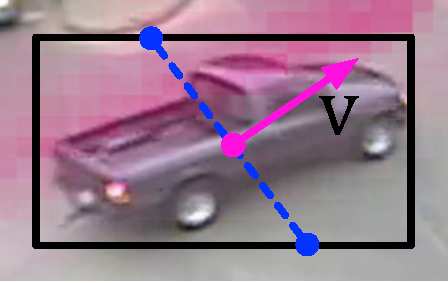
\includegraphics[width=\linewidth]{./img/semantic_tracker/box_perp_width.pdf}
    \subcaption{}
    \label{subfig:semantic-box-perp-width}
\end{subfigure}
\begin{subfigure}{0.27\linewidth}
    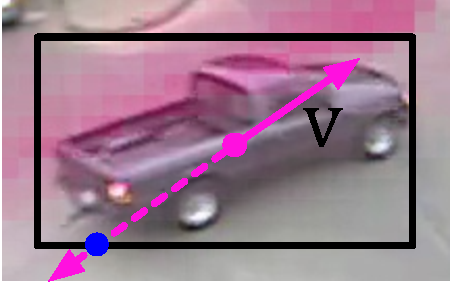
\includegraphics[width=\linewidth]{./img/semantic_tracker/last_pt.pdf}
    \subcaption{}
    \label{subfig:semantic-last-pt}
\end{subfigure}
\begin{subfigure}{0.42\linewidth}
    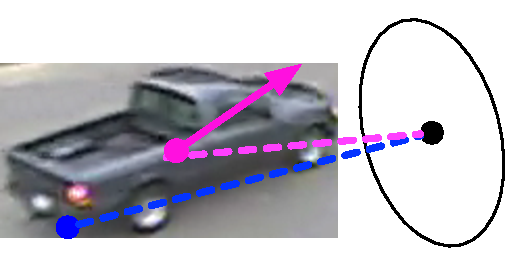
\includegraphics[width=\linewidth]{./img/semantic_tracker/last_pt_dist.pdf}
    \subcaption{}
    \label{subfig:semantic-last-pt-dist}
\end{subfigure}%
\caption{All the solid pink arrows above indicate the moving direction $\bm{v_r}$, the pink dot is the center of the rectangle, blue dots are the intersection points with the rectangle. (\subref{subfig:semantic-box-perp-width}): perpendicular width $W(\bm{r}, \bm{v_r})$ of the object's bounding box wrt. to  direction $\bm{v}_{r}$, shown as the blue dash line. \subref{subfig:semantic-last-pt}: last point $P(\bm{r}, \bm{v_r})$ of the object's bounding box $\bm{r}$, where the dash arrow is $R(\bm{r}, \bm{-v_r})$. (\subref{subfig:semantic-last-pt-dist}): distance between a hotspot with a rectangle's center point and last point $P(\bm{r}, \bm{v_r})$, shown in pink and blue dash lines.}
\label{fig:semantic-perp-width}
\end{figure}